\documentclass[letterpaper, 12pt]{article}

%%%%%%%%%%%%%%%%%%%%%%%%%%%%%
% DEFINITIONS
% Change those informations
% If you need umlauts you have to escape them, e.g. for an ü you have to write \"u
\gdef\mytitle{Laborprotokoll}
\gdef\mythema{DezSys04}

\gdef\mysubject{Systemtechnik-Labor}
\gdef\mycourse{5BHIT 2015/16, Gruppe Z}
\gdef\myauthor{Michael Weinberger}

\gdef\myversion{1.0}
\gdef\mybegin{08. Januar 2016}
\gdef\myfinish{14. Januar 2016}

\gdef\mygrade{Note:}
\gdef\myteacher{Betreuer: Th.Micheler}
%
%%%%%%%%%%%%%%%%%%%%%%%%%%%%%

\input special/preamble.tex

\let\tempsection\section
\renewcommand\section[1]{\vspace{-0.3cm}\tempsection{#1}\vspace{-0.3cm}}
\WithSuffix\newcommand\section*[1]{\tempsection*{#1}}

\let\tempsubsection\subsection
\renewcommand\subsection[1]{\vspace{0cm}\tempsubsection{#1}\vspace{0cm}}

\let\tempsubsubsection\subsubsection
\renewcommand\subsubsection[1]{\vspace{0cm}\tempsubsubsection{#1}\vspace{0cm}}

\linespread{0.94}

\lhead{\mysubject}
\chead{}
\rhead{\bfseries\mythema}
\lfoot{\mycourse}
\cfoot{\thepage}
% Creative Commons license BY
% http://creativecommons.org/licenses/?lang=de
\rfoot{\ccby\hspace{2mm}\myauthor}
\renewcommand{\headrulewidth}{0.4pt}
\renewcommand{\footrulewidth}{0.4pt}

\begin{document}
\parindent 0pt
\parskip 6pt

\pagenumbering{Roman} 
%!TEX root=../laborprotokoll.tex

\begin{titlepage}

	\begin{figure}[!h]
		\begin{flushright}
			
\includegraphics[width=0.3\linewidth]{images/jdIT_tgm.png}
		\end{flushright}
	\end{figure}

	\vspace{2.5cm} 

	{\begin{center} \bfseries\huge
			\rule{17.5cm}{0.1mm}  
			\\[5mm]
			\mytitle\\[5mm]
			\mythema\\
			\rule{17.5cm}{0.1mm}  
	\end{center}}

	{\begin{flushright} \bfseries\Large
			\vspace{2cm}
			\mysubject\\
			\mycourse\\[10mm]
			\myauthor\\[10mm]
	\end{flushright}}

	{\begin{table}[!h] \bfseries\normalsize
		\begin{tabularx}{\textwidth}{lXr @{\hspace{0mm}}}
			&& Version \myversion\\
			\mygrade && Begonnen am \mybegin\\
			\myteacher && Beendet am \myfinish\\
		\end{tabularx}
	\end{table}}

\end{titlepage}


\clearpage
\thispagestyle{empty}
\tableofcontents

\newpage
\pagenumbering{arabic}
\pagestyle{fancy}

%\vspace{-0.5cm}
\section{Einführung}
Diese Übung soll zur Vertiefung der Begriffe "Authentifizierung und Autorisierung" dienen.
\subsection{Ziele}
Das Ziel dieser Übung ist die Funktionsweise eines Verzeichnisdienstes zu verstehen und Erfahrungen mit der Administration auszuprobieren. Ebenso soll die Verwendung des Dienstes aus einer Anwendung heraus mit Hilfe der JNDI geübt werden. \newline
Authentifizierung bedeutet hier, dass per Username und Passwort eine Anmeldung beim Verzeichnisdienst erfolgt. Autorisierung wird hier im Zusammenhang mit Service-Gruppen und zugeordneten Usern durchgeführt.
\subsection{Voraussetzungen}
\begin{itemize}
	\item Grundlagen Verzeichnisdienst
	\item Administration eines LDAP Dienstes
	\item Verwendung von Commandline Werkzeugen fuer LDAP (LDAPSEARCH, LDAPMODIFY)
	\item Grundlagen der JNDI API für eine JAVA Implementierung
	\item Verwendung einer virtuellen Instanz für den Betrieb des Verzeichnisdienstes
\end{itemize}
\subsection{Aufgabenstellung}
Mit Hilfe der zur Verfuegung gestellten VM wird ein vorkonfiguriertes LDAP Service zur Verfuegung gestellt. Dieser Verzeichnisdienst soll um folgende Eintraege erweitert werden. Das verwendete Namensschema (eg. group.service1 oder vorname.nachname) soll fuer alle Eintraege verwendet werden.
\begin{itemize}
	\item 5 Posix Groups (beliebe Zuweisung von UserIDs)
	\item 10 User Accounts
\end{itemize}
Weiters soll eine Java-Applikationen zur Authentifizierung und Autorisierung entwickelt werden. Folgende Fragestellungen stehen dabei im Mittelpunkt:
\begin{itemize}
	\item Sind Username und Passwort korrekt? 
(Identifikation des Benutzers)
	\item Ist der User berechtigt ein bestimmtes Service zu nutzen?
(Benutzer-Berechtigung)
\end{itemize}
\newpage

\section{Dokumentation der Arbeitsschritte}
\subsection{Grundkonfiguration}
Folgendes Textfile von Prof. Micheler beschreibt das Aufsetzen eines OpenLDAP-Servers, die Grundkonfiguration, Grundlagen in LDAPSEARCH sowie LDAPMODIFY und listet einige weiterführende Links auf. \newline
\begin{lstlisting}[frame=single, caption=Grundkonfiguration]
Installation LDAP:
------------------
sudo apt-get update
sudo apt-get install slapd ldap-utils

sudo dpkg-reconfigure slapd
> DNS domain name: nodomain.com
> Organization name: nodomain
> Administrator password: user
> Database backend: hdb

Installation phpLDAPadmin:
--------------------------
sudo apt-get install phpldapadmin

Configuration phpLDAPadmin:
---------------------------
sudo gedit /etc/phpldapadmin/config.php

$servers->setValue('server','host','localhost');
$servers->setValue('server','base',array('dc=nodomain,dc=com'));
$servers->setValue('login','bind_id','cn=admin,dc=nodomain,dc=com');
$config->custom->appearance['hide_template_warning'] = true;

SSL configuration not performed!

Configuration Apache:
---------------------
/etc/apache2/mods-enabled/alias.conf: following line added
Alias /ldap /usr/share/phpldapadmin/htdocs

Link to phpLDAPadmin:
---------------------
http://localhost/ldap

Modify LDAP Directory:
----------------------
Add new Posix Group: group.default
Add new Posix Group: group.service1
Add new Generic User Account: max.mustermann
Add max.mustermann to group.service1

LDAPSEARCH Commandline Tool / Local:
------------------------------------
ldapsearch -h 127.0.0.1 -p 389 -D "cn=admin,dc=nodomain,dc=com" -W
ldapsearch -h 127.0.0.1 -p 389 -D "cn=max.mustermann,dc=nodomain,dc=com" -W

LDAPSEARCH Commandline Tool / Remote:
-------------------------------------
ldapsearch -h 192.168.0.8 -p 389 -D "cn=admin,dc=nodomain,dc=com" -W
ldapsearch -h 192.168.0.8 -p 389 -D "cn=max.mustermann,dc=nodomain,dc=com" -W -b "dc=nodomain,dc=com"
ldapsearch -h 192.168.0.8 -p 389 -D "cn=max.mustermann,dc=nodomain,dc=com" -W -b "cn=group.service2,dc=nodomain,dc=com" memberUid
ldapsearch -h 192.168.0.8 -p 389 -D "cn=max.mustermann,dc=nodomain,dc=com" -W -b "dc=nodomain,dc=com" "cn=group.*" memberUid
ldapsearch -h 192.168.0.8 -p 389 -D "cn=max.mustermann,dc=nodomain,dc=com" -W -b "dc=nodomain,dc=com" "(objectclass=PosixGroup)"

\end{lstlisting}
\newpage
\begin{lstlisting}[frame=single, caption=Grundkonfiguration]
LDAPMODIFY Commandline Tool / Remote:
-------------------------------------
ldapmodify -h 192.168.0.8 -p 389 -D "cn=admin,dc=nodomain,dc=com" -W  
dn: cn=group.service1,dc=nodomain,dc=com             
changetype: modify
replace: description
description: test


Links:
------
http://docs.oracle.com/javase/tutorial/jndi/index.html
http://www.stefan-seelmann.de/media/presentations/JUGM2008_JavaUndLDAP.pdf
https://www.digitalocean.com/community/tutorials/how-to-install-and-configure-openldap-and-phpldapadmin-on-an-ubuntu-14-04-server
\end{lstlisting}

\subsection{Anlegen von 5 Gruppen und 10 User-Accounts}
In der beschriebenen Testumgebung ist die phpLDAPadmin-Oberfläche via \textit{http://localhost/ldap/} aufzurufen. Im Login-Screen meldet man sich per Credentials \\ \textit{cn=admin,dc=nodomain,dc=com} und \textit{user} an. In der Adminoberfläche findet sich im linken Menü der Eintrag 'Create new entry here'. Eine Liste an Templates für den Erstellungsprozess wird angezeigt, wir wählen zuerst 'Generic: Posix Group' aus. Die GID-Nummer wird automatisch generiert, der Gruppe kann auch ein Name gegeben werden, in unserem Fall 'service1' bis 'service5'. \\ \\
Um einen User zu erstellen findet sich unter 'Create new entry here' der Eintrag 'Generic: User Account'. Relevant bei der Eingabe ist der Vor- und Nachname, die GID-Nummer (zugehörige Gruppe) und das Passwort, der Rest wird automatisch generiert aus den bereitgestellten Daten, kann gegebenenfalls trotzdem noch angepasst werden. \\
\begin{figure}[h]
	\centering 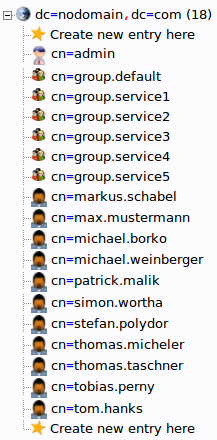
\includegraphics[keepaspectratio=true, scale=0.65]{images/10user5groups}
	\caption{10 User-Accounts, 5 Posix-Groups}
\end{figure}
\newpage
\subsection{LDAPSEARCH und LDAPMODIFY}
\subsubsection{LDAPSEARCH 1}
\begin{lstlisting}[frame=single, language=bash, caption=1.Befehl]
ldapsearch -h 127.0.0.1 -p 389 -D "cn=admin,dc=nodomain,dc=com" -w user
\end{lstlisting} 
Mit diesem Befehl wird erfolgreich ein Bind auf den Localhost-LDAP-Server (Port 389/TLS) durchgeführt, ohne Suchanfrage und ohne nennenswerte Ausgabe.
\subsubsection{LDAPSEARCH 2}
\begin{lstlisting}[frame=single, language=bash, caption=2.Befehl]
ldapsearch -h 192.168.128.136 -p 389 -D "cn=admin,dc=nodomain,dc=com" -w user
\end{lstlisting} 
Gleiches Vorgehen wie bei LDAPSEARCH 1, jedoch wird nun von 'außen' auf den LDAP-Server zugegriffen.
\subsubsection{LDAPSEARCH 3}
\begin{lstlisting}[frame=single, language=bash, caption=3.Befehl]
ldapsearch -h 192.168.128.136 -p 389 -D "cn=admin,dc=nodomain,dc=com" -w user -b "dc=nodomain,dc=com"
\end{lstlisting} 
Wieder ein Zugriff von außen, mithilfe von -b kann der Startpunkt der Suche angegeben werden, hier wird der gesamte Inhalt unserer Domäne ausgegeben.
\subsubsection{LDAPMODIFY 1}
\begin{lstlisting}[frame=single, language=bash, caption=4.Befehl]
ldapmodify -h 192.168.0.8 -p 389 -D "cn=admin,dc=nodomain,dc=com" -w user
dn: cn=michael.weinberger,dc=nodomain,dc=com
changetype: modify
replace: sn
sn: Mueller
\end{lstlisting} 
Zugriff von außen, der Nachname ('sn') wird per Befehl auf den Namen 'Müller' gesetzt.
\subsubsection{LDAPMODIFY 2}
\begin{lstlisting}[frame=single, language=bash, caption=5.Befehl]
ldapmodify -h 127.0.0.1 -p 389 -D "cn=admin,dc=nodomain,dc=com" -w user 
-f /home/user/Documents/SYT/data.ldif
\end{lstlisting} 
Lokaler Aufruf, liest anstatt von stdin die Änderungsinformationen aus einem LDIF-File (LDAP Data Interchange Format), das derselben Struktur entsprechen muss.
\newpage

\section{Authentifizierung}
Im Oracle JNDI Tutorial ist der Beispielcode implementiert worden, der für unsere Anwendung relevant ist. [1] \\
Via JOptionPane wird der User aufgefordert die Parameter einzugeben, ist daher nicht statisch und für jeden LDAP-Server, der unserem Aufbau ähnelt einsetzbar. Sofern der Bind auf den LDAP-Server geglückt ist, wird ein 'OK' ausgegeben, andernfalls 'NOK'.
\section{Autorisierung}
Um auch zu überprüfen, dass der User autorisiert ist (Mitglied einer Gruppe) wurde Sourcecode eines Forums bezogen [2]. Über 'SearchControls' (javax.naming.directory.SearchControls) kann in einem LDAP-Verzeichnis gesucht werden. Enthält die Gruppe das Attribut 'memberuid', so wird OK ausgegeben, andernfalls NOK.
\section{LDAP-Änderung mit bestimmten User}
Änderungen ohne Adminrechte lassen sich per ACL (Access Control List) definieren. In jener kann man bestimmte Rechte für Benutzer, Gruppen zuteilen. Diese Konfiguration muss in der slapd-Konfigurationsdatei \textit{/etc/ldap/slap.d} vorgenommen werden. \\
\begin{lstlisting}[frame=single, language=bash, caption=ACL]
access to dn.subtree="dc=example,dc=com" attrs=homePhone
        by self write
        by dn.children="dc=example,dc=com" search
        by peername.regex=IP:10\..+ read
    access to dn.subtree="dc=example,dc=com"
        by self write
        by dn.children="dc=example,dc=com" search
        by anonymous auth
\end{lstlisting} 
\newpage

\section{Quellen}
[1]: http://docs.oracle.com/javase/tutorial/jndi/ldap/examples/Simple.java, Oracle Documentation, zuletzt abgerufen am 14.01.2016 \newline
[2]: http://stackoverflow.com/questions/2172831/how-do-a-ldap-search-authenticate-against-this-ldap-in-java, leider Gottes Stack Overflow, zuletzt abgerufen am 14.01.2016 \\
\lstlistoflistings
\listoffigures

\end{document}
